\documentclass{article}

\usepackage{../preamble}
\standalonetrue

\pagestyle{fancy}
\fancyhf{}
\rhead{Section \thesection}
\lhead{PHYS 304 Lecture 1}
\rfoot{Page \thepage}


\title{PHYS 304 Lecture 1}
\author{Ashtan Mistal}
\date{!!!}

\begin{document}

\ifstandalone
\maketitle
\fi

\graphicspath{{./Lecture01/}}

\section{Introduciton}

\subsection{General Introduction Notes}

\begin{itemize}
    \item Canvas contains all the relevant information for the course. 
    \item Tutorial is Wednesday from 3:00 to 4:00 in HENN 202. 
\end{itemize}

Introductory Questions:

\begin{itemize}
    \item What does “quantum mechanics” mean to you?
    
    \begin{itemize}
        \item Open-ended question; multiple answers were shared. 
    \end{itemize}
    \item What distinguishes quantum mechanics from classical mechanics?
    \begin{itemize}
        \item Different equation of motion
        \item Fundamentally probabilistic behavior
        \item All entities have both particle and wavelike properties
        \item Energy is quantized
    \end{itemize}
    
    \item What technologies rely on quantum mechanics?
    
    \begin{itemize}
        \item Anything related to superconducting
        \item Atomic clocks
        \item MRI machines
        \item Quantum key distribution
    \end{itemize}

\end{itemize}

The course will fundamentally deal with the quantum mechanics of objects that are classically treated as particles. 

Professor Jeff Young's research is primarily focused in the quantum mechanical properties of light. 

\begin{itemize}
    \item Introduced to research. 
\end{itemize}

\subsection{Quantum Optics}

Are all of these examples of "classical light"?

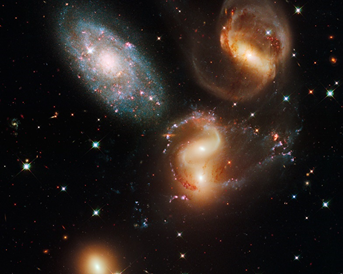
\includegraphics[width = 0.47 \textwidth]{Lecture01/1.png}
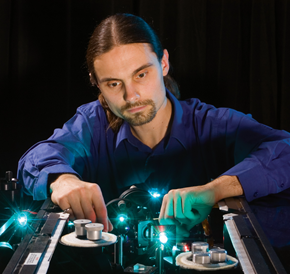
\includegraphics[width = 0.47 \textwidth]{Lecture01/2.png}


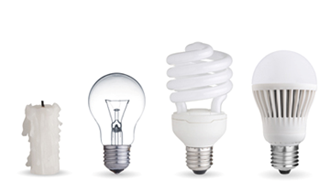
\includegraphics[width = 0.47 \textwidth]{Lecture01/3.png}
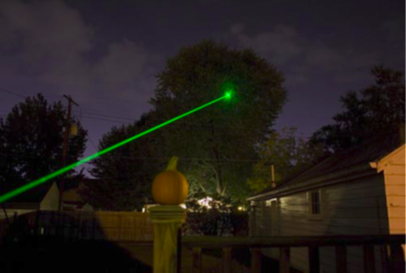
\includegraphics[width = 0.47 \textwidth]{Lecture01/4.png}

The source of the light, accelerating electrons, might require quantum mechanical treatment to fully understand, but the light itself can be described classically.



\begin{itemize}
    \item Gave example of double slit experiment; it can be simply understood using classical superposition of wave concepts. 
    \item Emphasized delocalized nature of waves and their superposition: the total wave everywhere in space and time is the sum of all constituent waves at all points in space and time. 
    \item Showed phet simulation of classical laser beam. 
    \item We can use quantum mechanics in laser light to describe the atoms, but simple classical mechanics to describe the light. 
    \item As we will learn, all objects have both wave-like and particle-like properties. 
    \item Therefore, although you don't need to think of a laser beam as a collection of photons you can nonetheless describe it in those terms. 
    \item ex: 50/50 beamsplitter
\end{itemize}

\section{Learning Goals}

\begin{enumerate}
    \item Identify when a problem requires a quantum mechanical solution. 
    \item Formulate a quantum mechanical approach to solving some simple problems. 
    \item Solve for the stationary states of some simple systems.
    \item Construct the full temporal and spatial evolution of a system’s wavefunction (the basic formalism).
    \item Solve some simple quantum mechanical problems analytically and numerically.
    \item Understand the nature of abstract Hilbert space and its relationship to “wavefunctions” defined with respect to different system variables.
    \item Understand the defining characteristics of the stationary quantum mechanical states of the hydrogen atom.

\end{enumerate}

\end{document}